\section*{Condo}

\subsection*{Create new condo}

\begin{itemize}
  \item[] \textbf{Trigger:} User interaction with CMS window
  \item[] \textbf{Precondition:} Assert that user has logged in
  \item[] \textbf{Path:}
    \begin{enumerate}
      \item User clicks Admin on navigation bar
      \item User clicks on Condos in the dropdown
      \item User clicks ``New Condo'' button
      \item User fills the condo information in the form
      \item User clicks ``Create Condo'' button
      \item ``Condo successfully created'' message is shown together with the data
    \end{enumerate}
  \item[] \textbf{Requirements:}
    \begin{enumerate}
      \item The new condo's data should be added to the database
      \item The new condo's information should be displayed in the homepage correctly
      \item The condos' information should be listed in the creation order
    \end{enumerate}
  \item[] \textbf{Screenshots:} \\
    \includegraphics[scale=0.25]{./images/ss/condo/create/1.png}
    \includegraphics[scale=0.25]{./images/ss/condo/create/2.png}\\
    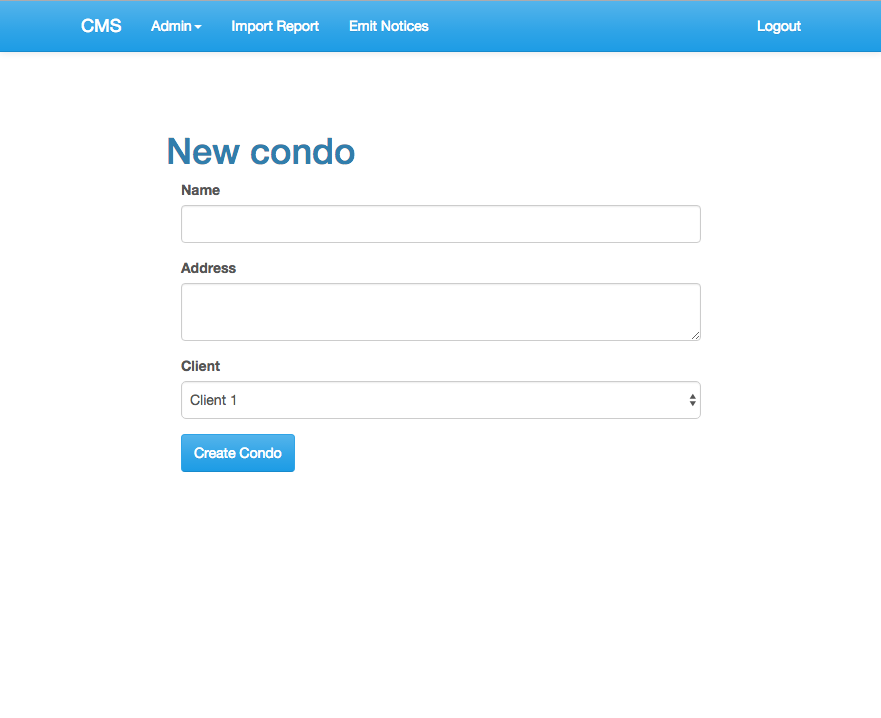
\includegraphics[scale=0.25]{./images/ss/condo/create/3.png}
    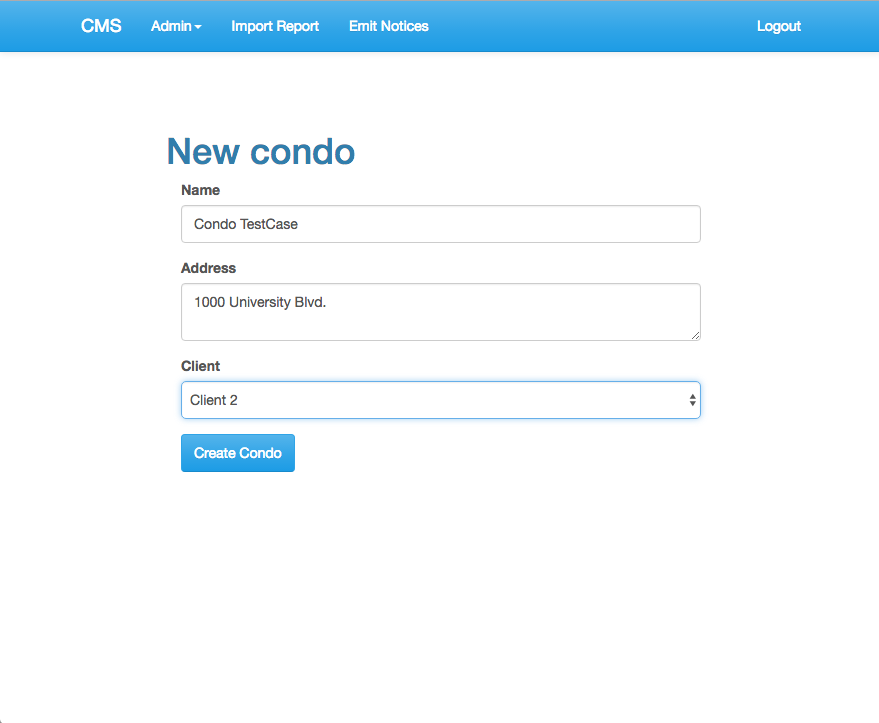
\includegraphics[scale=0.25]{./images/ss/condo/create/4.png}\\
    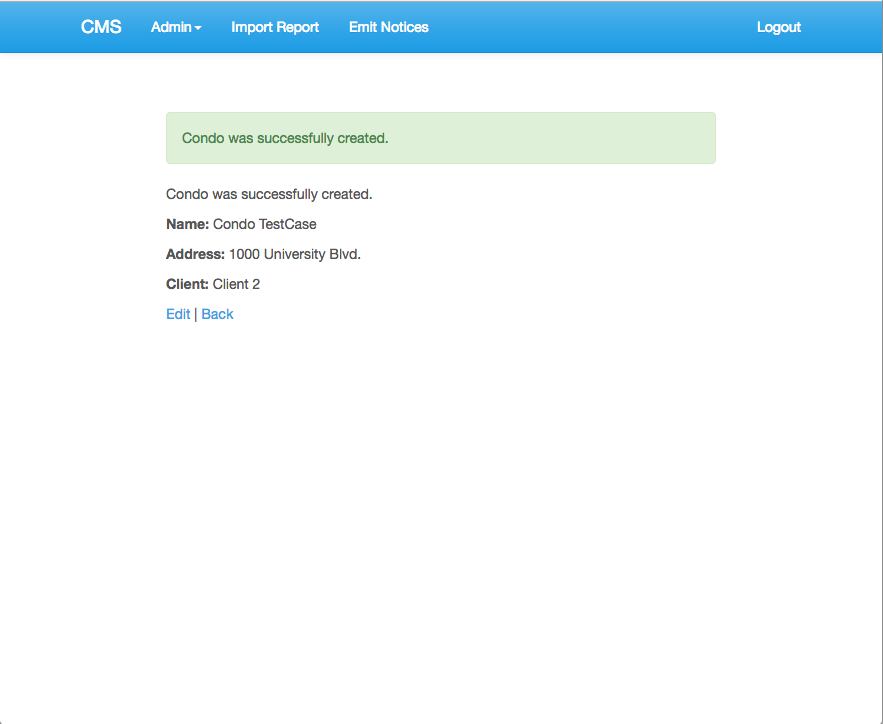
\includegraphics[scale=0.25]{./images/ss/condo/create/5.png}
\end{itemize}

\subsection*{Edit a condo}

\begin{itemize}
  \item[] \textbf{Trigger:} User interaction with CMS window
  \item[] \textbf{Precondition:} Assert that user is in the Condo page and the condo to edit is existed
  \item[] \textbf{Path:}
    \begin{enumerate}
      \item User clicks on Edit behind the information of the condo who will be edited
      \item User edit new information in the form
      \item User clicks ``Update Condo'' button
      \item ``Condo successfully updated'' massage is shown
    \end{enumerate}
  \item[] \textbf{Requirements:}
    \begin{enumerate}
      \item The updated condo’s new data should be updated to the database
      \item The updated condo’s new information should be displayed in the homepage correctly
      \item The condos’ information should be listed in the modification order
    \end{enumerate}
  \item[] \textbf{Screenshots:}\\
    \includegraphics[scale=0.25]{./images/ss/condo/edit/1.png}
    \includegraphics[scale=0.25]{./images/ss/condo/edit/2.png}\\
    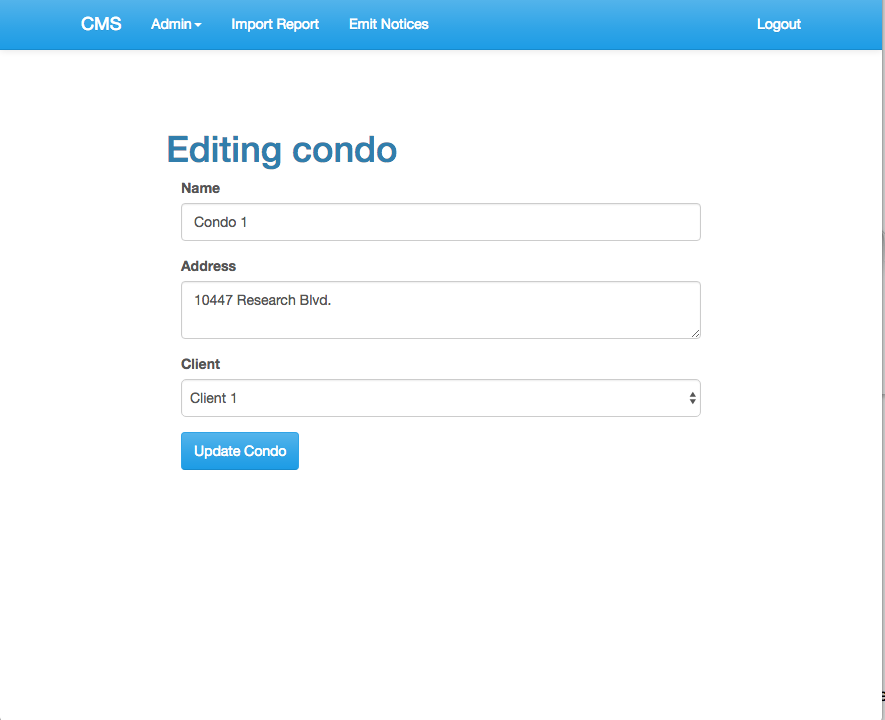
\includegraphics[scale=0.25]{./images/ss/condo/edit/3.png}
    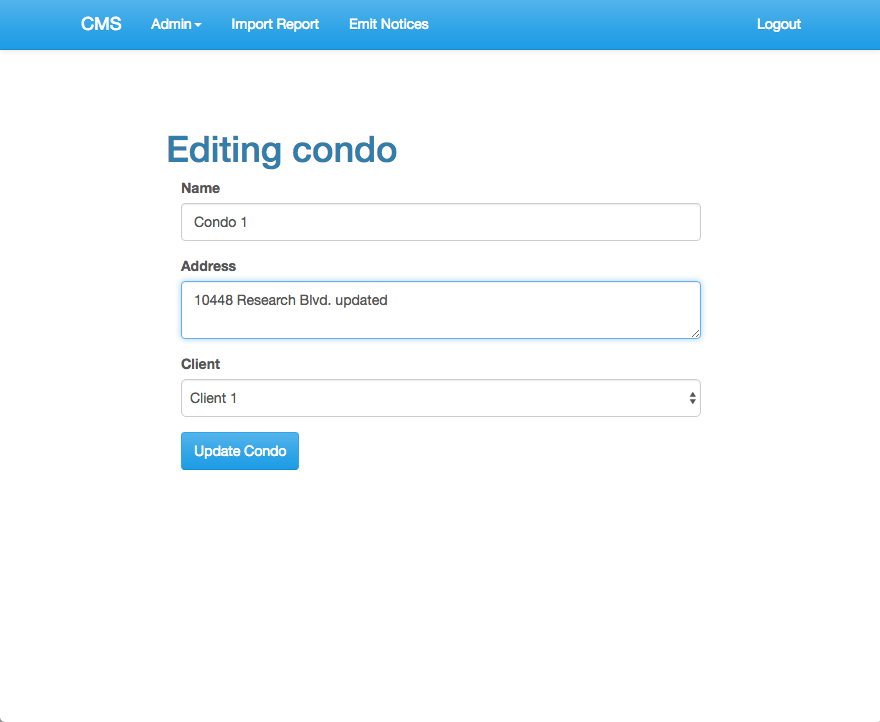
\includegraphics[scale=0.25]{./images/ss/condo/edit/4.png}\\
    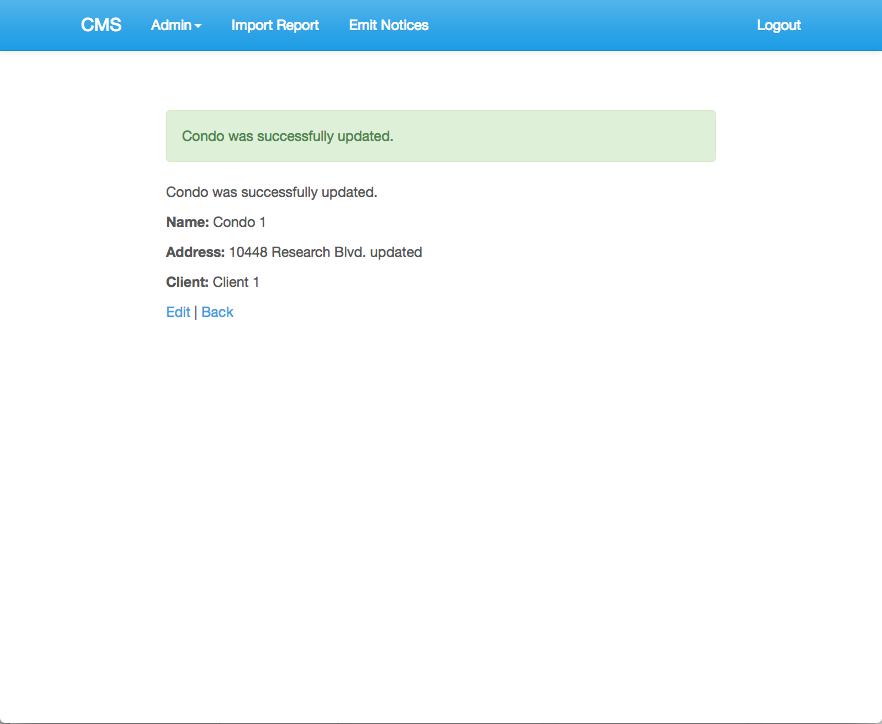
\includegraphics[scale=0.25]{./images/ss/condo/edit/5.png}
\end{itemize}

\subsection*{Delete a condo}

\begin{itemize}
  \item[] \textbf{Trigger:} User interaction with CMS window
  \item[] \textbf{Precondition:} Assert that user is in the Condo page and the condo to edit is existed
  \item[] \textbf{Path:}
    \begin{enumerate}
      \item User clicks on Destroy at the end of the information of the condo who will be deleted
      \item An alter message says ``Are you sure'' is shown
      \item User clicks ``OK'' button
      \item Condo successfully destroyed massage is shown
    \end{enumerate}
  \item[] \textbf{Requirements:}
    \begin{enumerate}
      \item The deleted condo’s data should be removed to the database
      \item The deleted condo’s information should not be displayed in the homepage
      \item Other condos’ information should be listed as the same as those before deleting
    \end{enumerate}
  \item[] \textbf{Screenshots:}\\
    \includegraphics[scale=0.25]{./images/ss/condo/delete/1.png}
    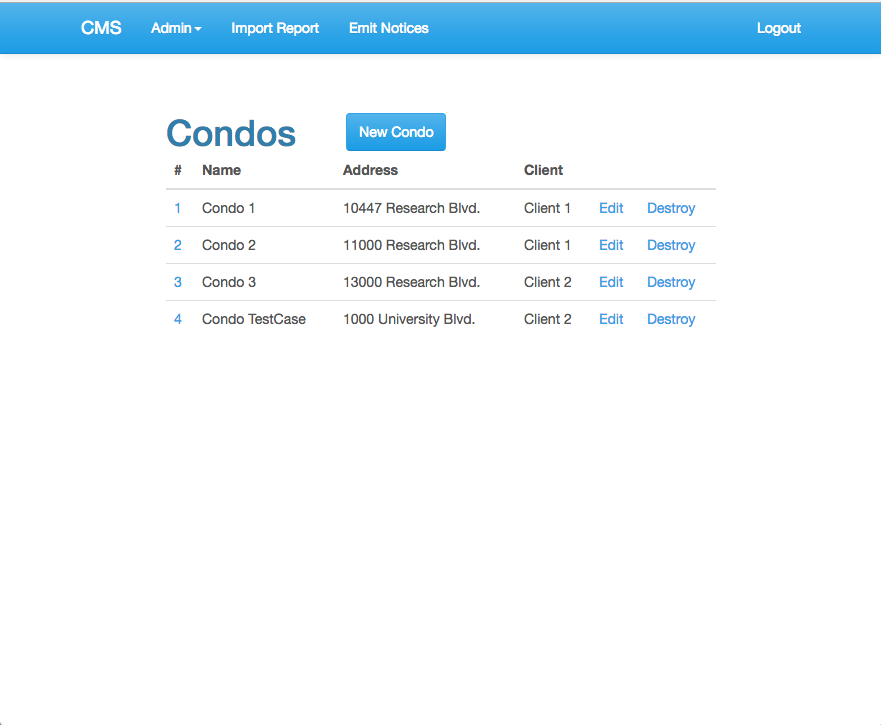
\includegraphics[scale=0.25]{./images/ss/condo/delete/2.png}\\
    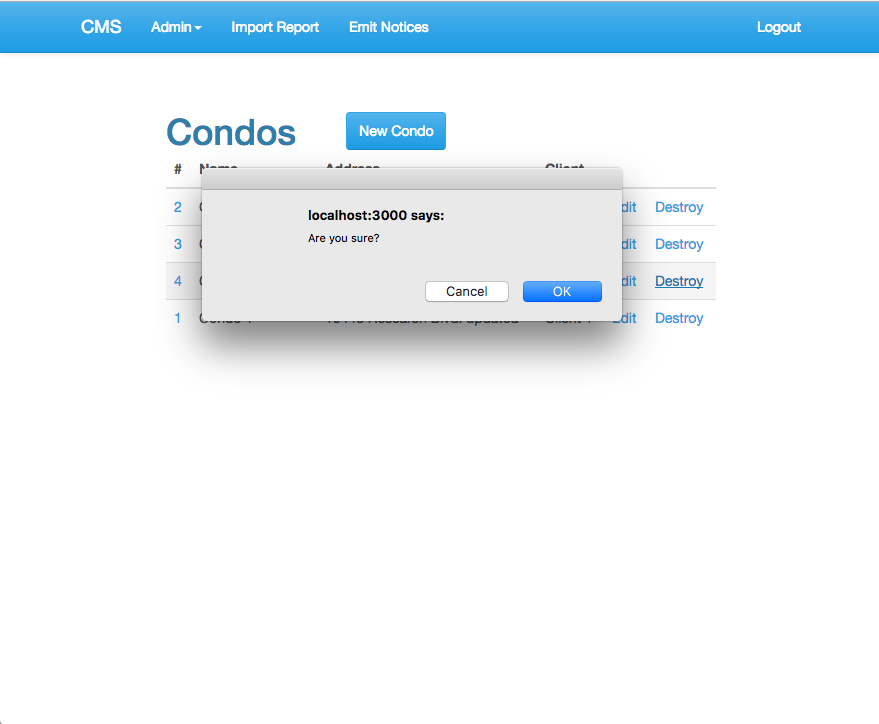
\includegraphics[scale=0.25]{./images/ss/condo/delete/3.png}
    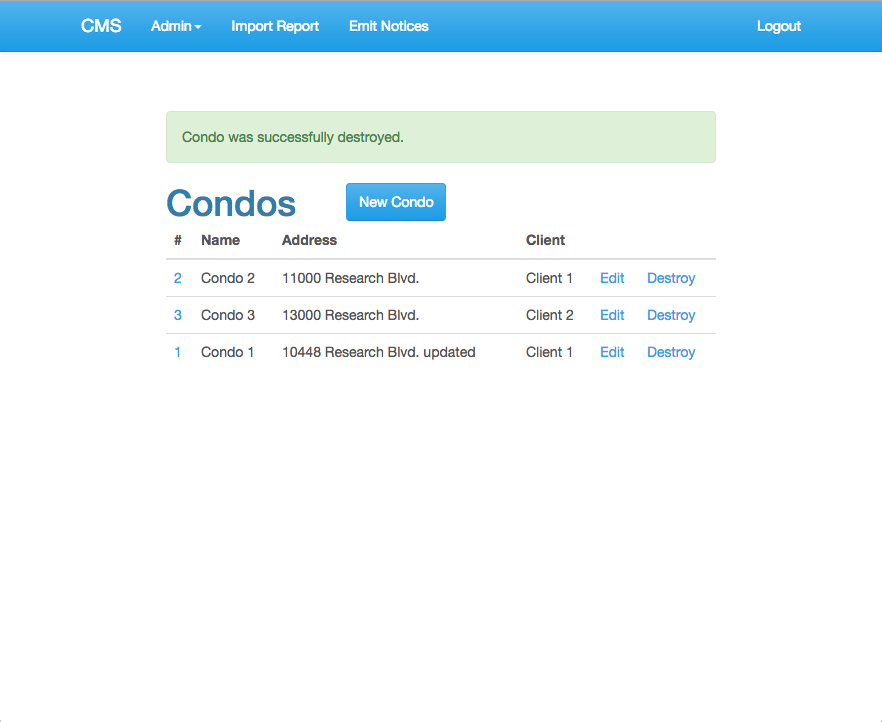
\includegraphics[scale=0.25]{./images/ss/condo/delete/4.png}
\end{itemize}
